% Options for packages loaded elsewhere
\PassOptionsToPackage{unicode}{hyperref}
\PassOptionsToPackage{hyphens}{url}
\PassOptionsToPackage{dvipsnames,svgnames,x11names}{xcolor}
%
\documentclass[
  letterpaper,
  DIV=11,
  numbers=noendperiod]{scrartcl}

\usepackage{amsmath,amssymb}
\usepackage{lmodern}
\usepackage{iftex}
\ifPDFTeX
  \usepackage[T1]{fontenc}
  \usepackage[utf8]{inputenc}
  \usepackage{textcomp} % provide euro and other symbols
\else % if luatex or xetex
  \usepackage{unicode-math}
  \defaultfontfeatures{Scale=MatchLowercase}
  \defaultfontfeatures[\rmfamily]{Ligatures=TeX,Scale=1}
\fi
% Use upquote if available, for straight quotes in verbatim environments
\IfFileExists{upquote.sty}{\usepackage{upquote}}{}
\IfFileExists{microtype.sty}{% use microtype if available
  \usepackage[]{microtype}
  \UseMicrotypeSet[protrusion]{basicmath} % disable protrusion for tt fonts
}{}
\makeatletter
\@ifundefined{KOMAClassName}{% if non-KOMA class
  \IfFileExists{parskip.sty}{%
    \usepackage{parskip}
  }{% else
    \setlength{\parindent}{0pt}
    \setlength{\parskip}{6pt plus 2pt minus 1pt}}
}{% if KOMA class
  \KOMAoptions{parskip=half}}
\makeatother
\usepackage{xcolor}
\usepackage[left=1in,right=1in,top=1in]{geometry}
\setlength{\emergencystretch}{3em} % prevent overfull lines
\setcounter{secnumdepth}{-\maxdimen} % remove section numbering
% Make \paragraph and \subparagraph free-standing
\ifx\paragraph\undefined\else
  \let\oldparagraph\paragraph
  \renewcommand{\paragraph}[1]{\oldparagraph{#1}\mbox{}}
\fi
\ifx\subparagraph\undefined\else
  \let\oldsubparagraph\subparagraph
  \renewcommand{\subparagraph}[1]{\oldsubparagraph{#1}\mbox{}}
\fi


\providecommand{\tightlist}{%
  \setlength{\itemsep}{0pt}\setlength{\parskip}{0pt}}\usepackage{longtable,booktabs,array}
\usepackage{calc} % for calculating minipage widths
% Correct order of tables after \paragraph or \subparagraph
\usepackage{etoolbox}
\makeatletter
\patchcmd\longtable{\par}{\if@noskipsec\mbox{}\fi\par}{}{}
\makeatother
% Allow footnotes in longtable head/foot
\IfFileExists{footnotehyper.sty}{\usepackage{footnotehyper}}{\usepackage{footnote}}
\makesavenoteenv{longtable}
\usepackage{graphicx}
\makeatletter
\def\maxwidth{\ifdim\Gin@nat@width>\linewidth\linewidth\else\Gin@nat@width\fi}
\def\maxheight{\ifdim\Gin@nat@height>\textheight\textheight\else\Gin@nat@height\fi}
\makeatother
% Scale images if necessary, so that they will not overflow the page
% margins by default, and it is still possible to overwrite the defaults
% using explicit options in \includegraphics[width, height, ...]{}
\setkeys{Gin}{width=\maxwidth,height=\maxheight,keepaspectratio}
% Set default figure placement to htbp
\makeatletter
\def\fps@figure{htbp}
\makeatother

\setkomafont{author}{\small}
\setkomafont{date}{\small}
\KOMAoption{captions}{tableheading}
\makeatletter
\makeatother
\makeatletter
\makeatother
\makeatletter
\@ifpackageloaded{caption}{}{\usepackage{caption}}
\AtBeginDocument{%
\ifdefined\contentsname
  \renewcommand*\contentsname{Table of contents}
\else
  \newcommand\contentsname{Table of contents}
\fi
\ifdefined\listfigurename
  \renewcommand*\listfigurename{List of Figures}
\else
  \newcommand\listfigurename{List of Figures}
\fi
\ifdefined\listtablename
  \renewcommand*\listtablename{List of Tables}
\else
  \newcommand\listtablename{List of Tables}
\fi
\ifdefined\figurename
  \renewcommand*\figurename{Figure}
\else
  \newcommand\figurename{Figure}
\fi
\ifdefined\tablename
  \renewcommand*\tablename{Table}
\else
  \newcommand\tablename{Table}
\fi
}
\@ifpackageloaded{float}{}{\usepackage{float}}
\floatstyle{ruled}
\@ifundefined{c@chapter}{\newfloat{codelisting}{h}{lop}}{\newfloat{codelisting}{h}{lop}[chapter]}
\floatname{codelisting}{Listing}
\newcommand*\listoflistings{\listof{codelisting}{List of Listings}}
\makeatother
\makeatletter
\@ifpackageloaded{caption}{}{\usepackage{caption}}
\@ifpackageloaded{subcaption}{}{\usepackage{subcaption}}
\makeatother
\makeatletter
\@ifpackageloaded{tcolorbox}{}{\usepackage[many]{tcolorbox}}
\makeatother
\makeatletter
\@ifundefined{shadecolor}{\definecolor{shadecolor}{rgb}{.97, .97, .97}}
\makeatother
\makeatletter
\makeatother
\ifLuaTeX
  \usepackage{selnolig}  % disable illegal ligatures
\fi
\IfFileExists{bookmark.sty}{\usepackage{bookmark}}{\usepackage{hyperref}}
\IfFileExists{xurl.sty}{\usepackage{xurl}}{} % add URL line breaks if available
\urlstyle{same} % disable monospaced font for URLs
\hypersetup{
  pdftitle={Hypothesis testing},
  pdfauthor={Practice problems},
  colorlinks=true,
  linkcolor={blue},
  filecolor={Maroon},
  citecolor={Blue},
  urlcolor={Blue},
  pdfcreator={LaTeX via pandoc}}

\title{Hypothesis testing}
\author{Practice problems}
\date{10/14/24}

\begin{document}
\maketitle
\ifdefined\Shaded\renewenvironment{Shaded}{\begin{tcolorbox}[breakable, enhanced, boxrule=0pt, frame hidden, borderline west={3pt}{0pt}{shadecolor}, interior hidden, sharp corners]}{\end{tcolorbox}}\fi

\begin{enumerate}
\def\labelenumi{\arabic{enumi}.}
\item
  For each of the research statements below, determine whether it
  represents a null hypothesis claim or an alternative hypothesis claim.

  \begin{enumerate}
  \def\labelenumii{\alph{enumii}.}
  \item
    The number of hours that grade-school children spend doing homework
    predicts their future success on standardized tests.
  \item
    King cheetahs on average run the same speed as standard spotted
    cheetahs.
  \item
    For a particular student, the probability of correctly answer a
    5-option multiple choice test is larger than 0.2 (i.e.~better than
    guessing)
  \item
    The probability of getting in a car accident is the same if using a
    cell phone then if not using a cell phone.
  \end{enumerate}
\item
  Write out the null and alternative hypotheses in words and also in
  statistical notation for each of the following situations. When
  writing in statistical notation, be sure to define quantities in
  context.

  \begin{enumerate}
  \def\labelenumii{\alph{enumii}.}
  \item
    New York is known as ``the city that never sleeps''. A random sample
    of 25 New Yorkers were asked how much they sleep they get per night.
    Does these data providing convincing evidence that New Yorkers on
    average sleep less than 8 hours per night?
  \item
    A study suggests that 25\% of 25 year-olds have gotten married. You
    believe that this is incorrect and decide to collect your own data
    to conduct a hypothesis test.
  \end{enumerate}
\item
  A Survey USA poll conducted in Seattle, WA in May 2021 reports that of
  the 650 respondents (adults living in this area), 159 support
  proposals to defund police departments.

  \begin{enumerate}
  \def\labelenumii{\alph{enumii}.}
  \item
    A journals writing a news story on the poll results wants to use the
    headline: ``More than 1 in 5 adults living in Seattle support
    proposals to defund police departments''. You caution the journalist
    that they should first conduct a hypothesis test to see if the poll
    data provide convincing evidence for this claim. Write the
    hypotheses for this test using proper notation, defining any
    necessary quantities.
  \item
    Describe in words a simulation scheme that would be appropriate for
    this situation. Also describe how the p-value can be calculated
    using the simulation results.
  \item
    The histogram below shows the distribution of 1000 simulated
    proportions under \(H_{0}\). Estimate the p-value using the plot and
    use it to evaluate your hypotheses (i.e.~make a conclusion). Assume
    a significance level of 0.05.

    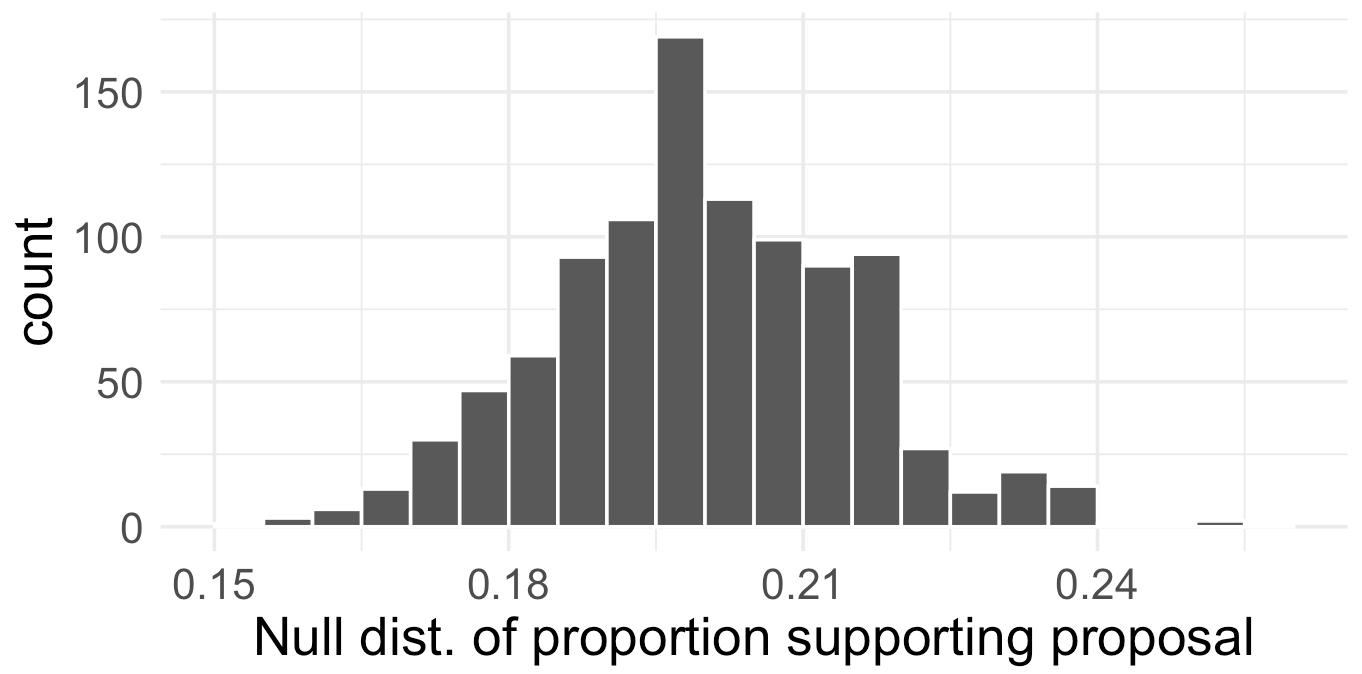
\includegraphics[width=4.05208in,height=\textheight]{images/13-defund.png}
  \end{enumerate}
\item
  \((^*)\) In a large university where 60\% of the full-time students
  are employed at least 5 hours per week, the members of the Statistics
  Department faculty wonder if the same proportion of their students
  work at least 5 hours per week. They randomly sample 25 of their
  majors and find that 12 of the students work 5 or more hours per week.

  Two sampling distributions were created to describe the variability in
  the proportion of statistics majors who work at least 5 hours per
  week: a null distribution and a bootstrap distribution. In both cases,
  \(B=1000\) simulations were generated.

  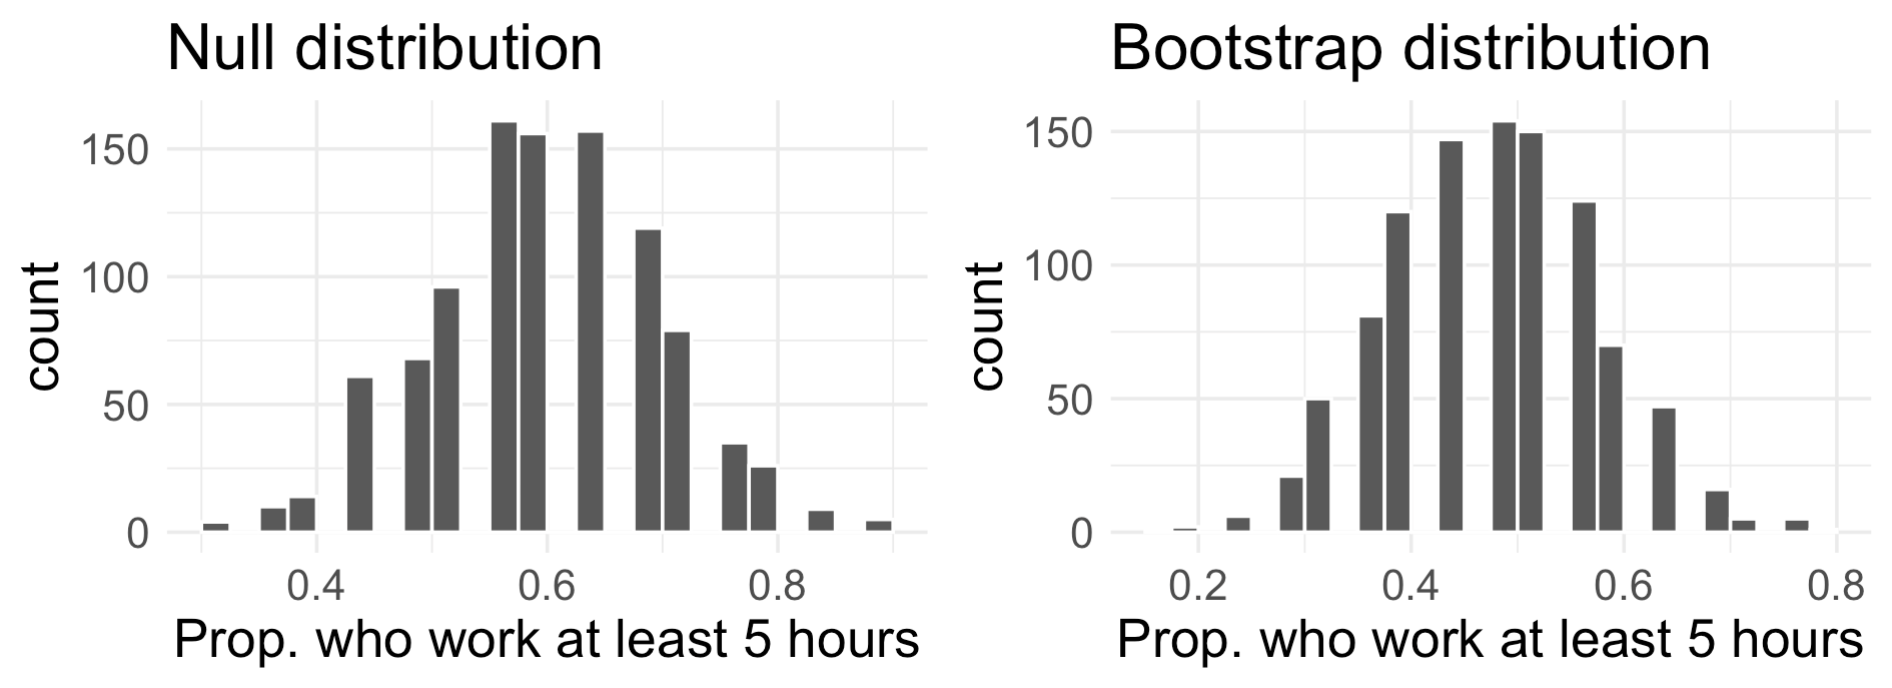
\includegraphics{images/13-hours.png}

  \begin{enumerate}
  \def\labelenumii{\alph{enumii}.}
  \item
    Which distribution(s) was/were obtained by sampling with
    replacement, and which distribution(s) was/were obtained by sampling
    without replacement?
  \item
    Estimate the standard error of the simulated proportions based on
    each distribution. Are the two standard errors you estimated roughly
    equal?
  \item
    Using the appropriate histogram, test the claim that 70\% of
    statistics majors, like their peers, work at least 5 hours per week.
    State the hypotheses, find the p-value, and conclude in the context
    of the problem. Use a significance level of 0.10.
  \item
    Using the appropriate histogram, find a 90\% bootstrap confidence
    interval for the true proportions of statistics majors who work at
    least 5 hours per week. Interpret the confidence interval in the
    context of the problem.
  \item
    Briefly comment on how your conclusions in (c) and (d) compare.
  \end{enumerate}
\item
  A study conducted in 2020 found that the U.S. adjusted divorce rate
  was 14 per 100 married women. Joe is suspicious and disagrees with the
  stated divorce rate. Joe somehow collected data from 323 married or
  previously-married women, and asked them if they had a divorce in
  2020. 55 of the women responded that they indeed had a divorce in
  2020.

  \begin{enumerate}
  \def\labelenumii{\alph{enumii}.}
  \item
    Write out the hypotheses corresponding to this scenario.
  \item
    Describe in words a simulation scheme that would be appropriate for
    this situation. Also describe how the p-value can be calculated
    using the simulation results.
  \item
    The histogram below shows the distribution of 1000 simulated
    proportions under \(H_{0}\). Estimate the p-value using the plot and
    use it to evaluate Joe's hypotheses (i.e.~make a conclusion). Assume
    a significance level of 0.05.

    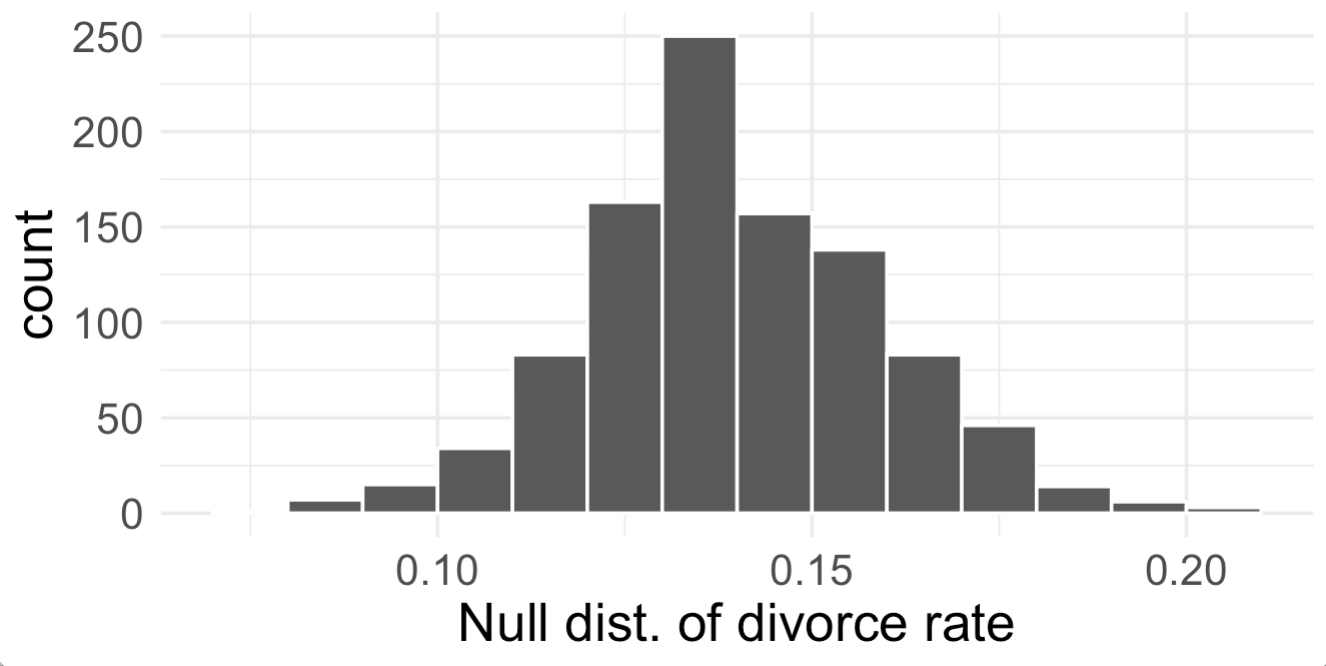
\includegraphics[width=4.54167in,height=\textheight]{images/13-divorce.png}
  \item
    Joe has some free time and also created a 90\% bootstrap confidence
    interval for the divorce rate.

    He obtained the following interval: (0.136, 0.204). Interpret this
    interval in context.
  \item
    Based on this interval, would it be appropriate for Joe to conclude
    that the study's reported rate was wrong? Explain your reasoning.
  \item
    How do your conclusions from (c) and (e) compare?
  \end{enumerate}
\end{enumerate}



\end{document}
